%%%%%%%%%%%%%%%%%%%%%%%%%%%%%%%%%%%
% Author: Dominic Heaton
% University of Southampton
% 2777 9009 - dhh1g15
%%%%%%%%%%%%%%%%%%%%%%%%%%%%%%%%%%%

\documentclass[a4paper,11pt]{article}

%%%%%%%%%%%%%%%%%%%%%%%%%%%%%%%%%%
% PACKAGES
%%%%%%%%%%%%%%%%%%%%%%%%%%%%%%%%%%
\usepackage[margin=1in]{geometry}
\usepackage{graphicx}
\usepackage{textgreek}
\usepackage{caption}
\usepackage{gensymb}
\renewcommand{\baselinestretch}{1.2} % line spacing
\usepackage{tikz}
\def\checkmark{\tikz\fill[scale=0.4](0,.35) -- (.25,0) -- (1,.7) -- (.25,.15) -- cycle;}
\usepackage{float}
\usepackage{color}
\usepackage{hyperref}
\usepackage[titletoc,title]{appendix}
\usepackage{pdfpages}
\usepackage{listings}
\lstset{language=python, basicstyle=\footnotesize, breaklines=true,showstringspaces=false, numbers=left, stepnumber=1, frame=single,}
\usepackage{chngcntr}
\counterwithout{figure}{section}
\setlength{\parindent}{0pt}
\setlength{\parskip}{2.0ex plus0.5ex minus0.2ex}
%%%%%%%%%%%%%%%%%%%%%%%%%%%%%%%%%%
% DOCUMENT BEGIN
%%%%%%%%%%%%%%%%%%%%%%%%%%%%%%%%%%
\begin{document}

%%%%%%%%%%%%%%%%%%%%%%%%%%%%%%%%%%
%Title Page

\begin{titlepage}

	\centering
	
	{\LARGE\bfseries ELEC6242: Cryptography \par}
	{\LARGE\bfseries Cryptanalysis Coursework \par}	

	\vspace{7cm}
	{\Large Dominic H. Heaton \par}
	
	\vspace{2cm}
	{\large\itshape Student ID: 2777 9009 \par}
	{\large\itshape dhh1g15@soton.ac.uk \par}
	{\large\itshape MEng Electronic Engineering with Mobile \& Secure Systems \par}
		
	\vfill
	{\scshape\LARGE University of Southampton \par}
	{\large \today \par}
	
\end{titlepage}

%%%%%%%%%%%%%%%%%%%%%%%%%%%%%%%%%%
%Start of Document
\tableofcontents
\pagebreak

\section{Outline} \label{Outline}
% which summarises the content of the reports
In this report various cryptanalysis methods are employed to decipher three ciphertexts each of which have been encrypted using different cipher methods. For each of the ciphertexts to be broken, a Python program was developed which was capable of producing the plaintext from the provided ciphertext as well as returning the value of the key used to encrypt the plaintext in the first place. The approach to deciphering each ciphertext is described in this report as well as the code developed being included for reference in the appendices.

\section{Solution for Cipher 1} \label{Solution for Cipher 1}
% this section only includes the plaintext for cipher 1 and the decryption key

{\bfseries{Deciphered Plaintext:}} 

Formative assessment can be viewed as a mean to enhance the learning process. Based on the results of such assessments, students will be able to assess their knowledge and identify strengths and weaknesses. The teacher will also have indication on how well the students are grasping the fundamental facts and whether he needs to alter their teaching to emphasis some important concepts.

{\bfseries{Key:}} tyu

\section{Cipher 1 Cryptanalysis} \label{Cipher 1 Cryptanalysis}
%  This section provides a summary of the techniques you have used to solve the cipher. It should include evidence of all analysis you have performed in order to solve the cipher such (e.g. frequency analysis), in addition it should refer to any programs you have developed in order to perform cryptanalysis (500 words)

	The first test of the ciphertext was to calculate the Index of Coincidence (IC). A python script, \url{indexOfCoincidence.py}, was generated to calculate the value as shown in Equation \ref{IoC}. The Index of Coincidence of 0.5278 is close to the value expected of written English (0.066) and therefore it was assumed that the plaintext was a message in English. From this value it was determined that the most likely ciphers to have been used to encrypt the message were substitutional ciphers.

		\begin{equation}
			IC\quad =\quad \frac { \sum _{ i=A }^{ Z }{ { f }_{ i }\left( { f }_{ i }-1 \right)  }  }{ N\left( N-1 \right)  } \quad =\quad 0.05278
			\label{IoC}
		\end{equation}
	
	The first decryption method attempted was the Caesar Substitutional Cipher, in which the letters in the plaintext will have been shifted by a fixed amount to generate the ciphertext. A Brute Force methodology was used in an attempt to decode the Caesar Cipher as in its simplest form there are only 25 possible keys. A script was generated (\url{caesar.py}) to output all of these possible deciphered plaintexts, but none of these revealed the message. 
	
	The next stage was then to attempt to decrypt the ciphertext using another substitutional cipher and therefore the Vigenere Cipher was selected. The approach for this cipher involved first carrying out the Kasisky Test to find the longest pattern of letters which were repeated within the ciphertext. The distance between these repetitions was then calculated, with the key length being a factor of this distance. This provided key lengths of \url{1, 2, 3, 6, 13, 26, 39, 78} given the distance of 78 characters between the repeated pattern \url{tqmxqmfchm}. It was assumed that the encryption key was unlikely to have a length less than 3 and therefore keys of length 1 and 2 were ignored.
	
	Frequency Analysis was carried out under the assumption of a key space of 3 letters, producing the graphs in Figure \ref{q1freq}. Each graph represents a letter of the key and compares the frequency of the letters in the ciphertext to that of the frequency of a letter appearing in the English language. The graphs allow the determination of the shift applied for each letter in the plaintext to generate the ciphertext. The first attempt to decipher the message using the shifts extracted from the frequency analysis provided the plaintext shown in Figure \ref{q1attempt}.

		\begin{figure}[h]
			\centering
			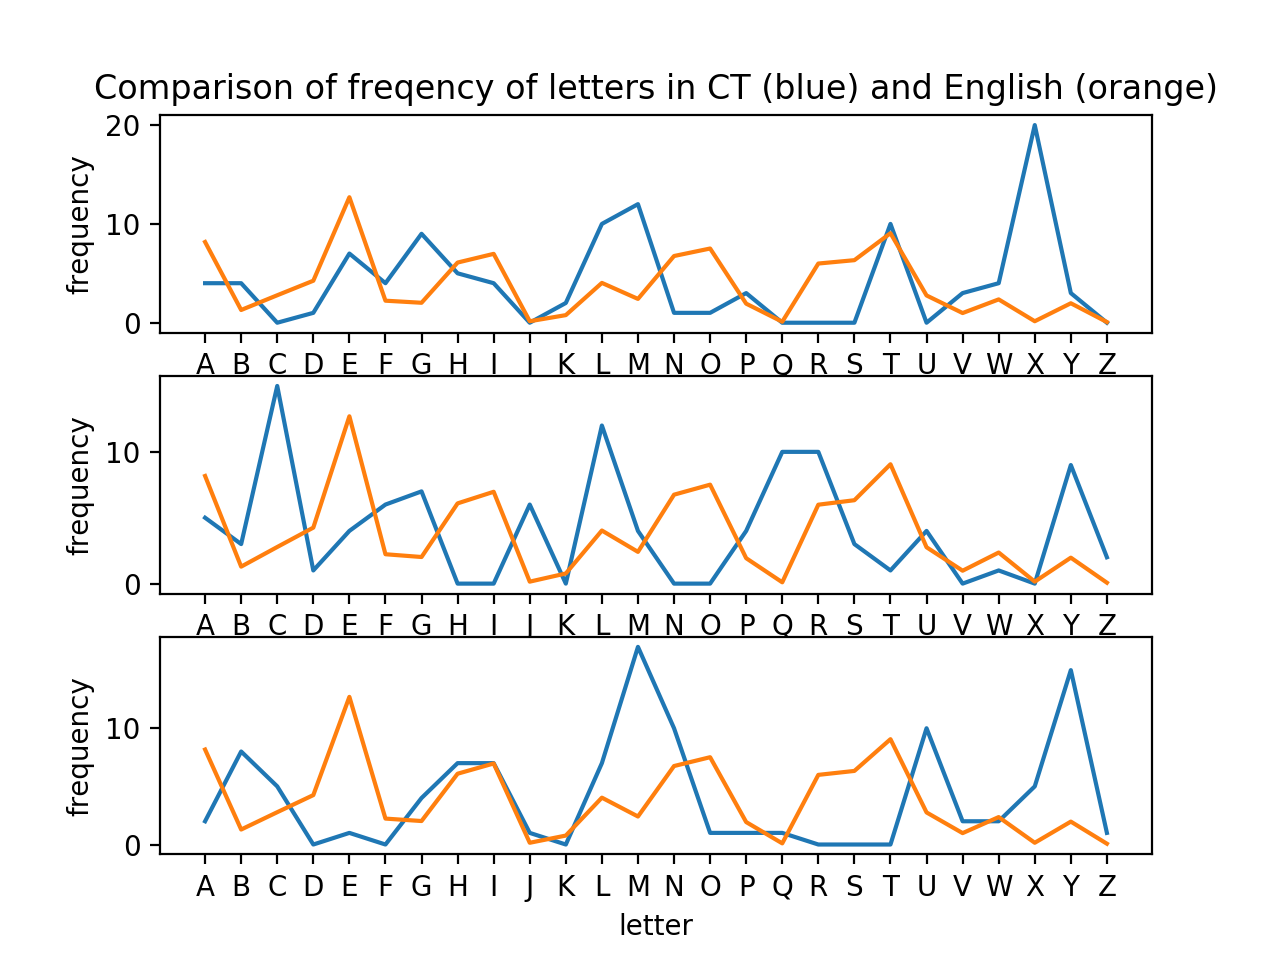
\includegraphics[width = 12cm]{img/q1freq}
			\captionsetup{width = 13cm}
			\caption{Frequency Analysis of the Ciphertext (CT) assuming a key space of 3 in the Vigenere Cipher. The shape of the curves on each graph allows the shift used in the Vigenere cipher to be determined. The graphs show the frequency of letters in the ciphertext (blue) and the english language (orange).}
			\label{q1freq}
		\end{figure}
		
		\begin{figure}[h]
			\centering
			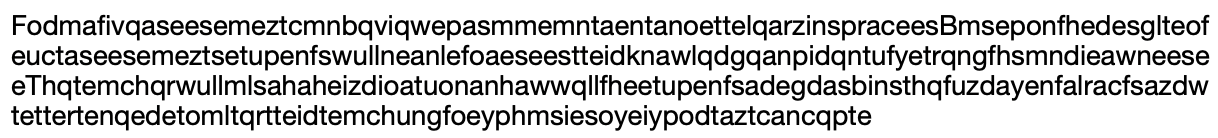
\includegraphics[width = 15cm]{img/q1attempt}
			\captionsetup{width = 13cm}
			\caption{First attempt at Vigenere Deciphering using a simple shift according to the most frequently appearing letters as shown in Figure \ref{q1freq}. The result resembles english except for every third letter has not been deciphered properly.}
			\label{q1attempt}
		\end{figure}	
		
	From Figure \ref{q1attempt} it can be seen that the Vigenere deciphering has revealed a plaintext which is almost a string of English words except for every third letter having been incorrectly deciphered. This meant that the shift used for the third letter of the key was incorrect. The third graph in Figure \ref{q1freq} shows several sharp peaks in frequency for the ciphertext. As the highest peak in the ciphertext proved unsuccessful in deciphering the plaintext, the next highest peak was used. This shift then allowed the plaintext to be revealed as shown in Section \ref{Solution for Cipher 1}. The key length of 3 had successfully deciphered the ciphertext, using the Vigenere Cipher. From these shifts it could be determined that the key is \url{tyu}. The \url{q3.py} script was generated to carry out the Vigenere Deciphering as well as the Kasisky Test and Frequency Analysis for this question. These scripts can be found in Appendix \ref{Code for solving Cipher 1}.
	
\section{Solution for Cipher 2} \label{Solution for Cipher 2}
% this section only includes the plaintext for cipher 2 and the decryption key
	{\bfseries{Deciphered Plaintext:}} 
	
	In ancient Egypt servants were smeared with honey to attract flies away from the pharaoh
	
	{\bfseries{Key:}} 0x1abc

\section{Cipher 2 Cryptanalysis} \label{Cipher 2 Cryptanalysis}		
% This section provides a summary of the techniques you have used to solve the cipher. It should include evidence of all analysis you have performed in order to solve the cipher, in addition it should refer to any programs you have developed in order to perform cryptanalysis (500 words)		
	
	This ciphertext was in the form of a `.hex' file and therefore a starting point was to look to decode the data into a read-able ASCII format to see if the message was encoded rather than encrypted into hexadecimal format. Figure \ref{hexToAscii} shows the `.hex' file alongside the ASCII representation showing that the message was not simply encoded. 
	
		\begin{figure}[h]
			\centering
			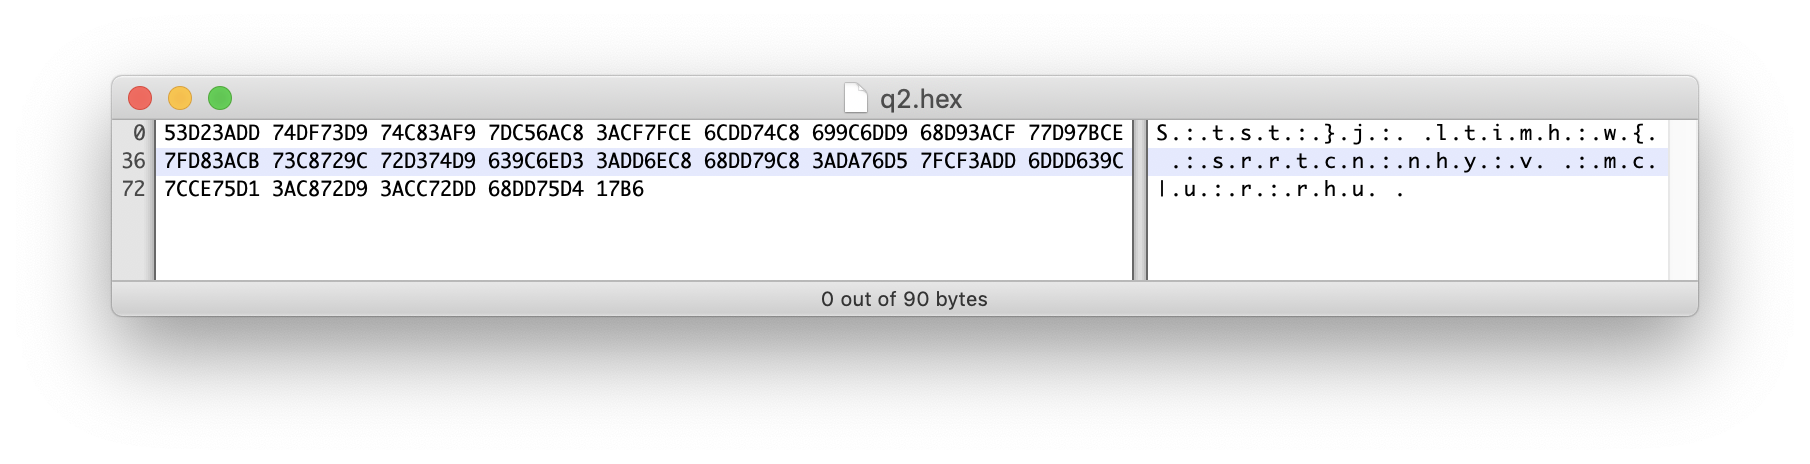
\includegraphics[width = 16cm]{img/hexToAscii}
			\captionsetup{width = 13cm}
			\caption{The hex file (left) to be decrypted in this question alongside the ASCII conversion (right) of the hexadecimal.}
			\label{hexToAscii}
		\end{figure}	
	
	The ciphertext is of hexadecimal form which is simply converted to binary at which point the XOR cipher seemed a reasonable cipher to start with in attempting to decipher the plaintext. This was because the XOR cipher is reversible and therefore the hint provided with the plaintext beginning with the letter `I' would allow a reverse engineering of the ciphertext to provide the key use to encrypt the plaintext.
	
	This method initially reverse engineered the first hexadecimal value in the ciphertext (\url{0x53}) to give the plaintext letter `I', giving the key to be \url{0x1a}. The XOR cipher applies the key to each byte of the plaintext until the message is encrypted (or decrypted). The 1-byte key of \url{0x1a} was applied to each byte of the ciphertext revealing the plaintext message shown in Figure \ref{q2attempt}. This plaintext revealed no meaningful information and therefore a key length of 1-byte was unsuccessful.
	
		\begin{figure}[h]
			\centering
			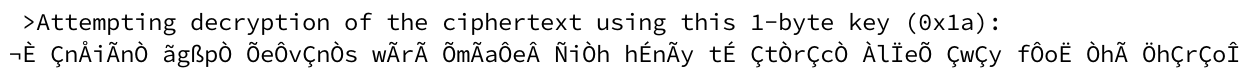
\includegraphics[width = 16cm]{img/q2attempt}
			\captionsetup{width = 13cm}
			\caption{Attempting to decipher the ciphertext using a 1-byte key of \url{0x1a} failed to produce a meaningful plaintext}
			\label{q2attempt}
		\end{figure}	
	
	Following the failure of a 1-byte key, an attempt to use a 2-byte key was used, where the first byte was the \url{0x1a} value which must be used for the first letter in the cipher as we know that the letter `I' is the first plaintext letter. A 2-byte key means that the bytes of the key are applied in an alternating pattern to bytes of the ciphertext (or plaintext as XOR is reversible).  
	
	The second byte of the key was found using the Brute Force methodology, where the key was of form \url{1aXX} where \url{XX} was the second byte of the key to be determined. If a second byte was found in this method, the plaintext would also be revealed at the same time. This brute force method iterated through all possible keys (00$\leq$XX$\leq$FF) to produce 256 plaintexts. English language detection was then applied on these plaintexts to extract only plaintexts which resembled english. This filter meant that the total number of plaintexts printed by the developed script was limited and from the shortened list produced, the actual plaintext and key could be easily spotted. The plaintext and key are shown in Section \ref{Solution for Cipher 2}. The python script (\url{q2.py}) developed to decipher the `.hex' file and reveal the plaintext and the key can be found in Appendix \ref{Code for solving Cipher 2}.
	
\section{Solution for Cipher 3} \label{Solution for Cipher 3}
%  this section only includes the plaintext for cipher 3 and the decryption key
	{\bfseries{Deciphered Plaintext:}} 
	
	There are probably more than hundred billion galaxies in the cosmos each of those has up to trillion stars
	
	{\bfseries{Key Length:}} 8

\section{Cipher 3 Cryptanalysis} \label{Cipher 3 Cryptanalysis}	
% This section provides a summary of the techniques you have used to solve the cipher. It should include evidence of all analysis you have performed in order to solve the cipher in addition it should refer to any programs you have developed in order to perform cryptanalysis (500 words).

	The first stage of deciphering the ciphertext was to carry out frequency analysis, producing the graph in Figure \ref{q3freq}. This figure shows a comparison of the frequency of letters appearing in the ciphertext in comparison to the frequency of letters appearing in the english language. The similar shapes of the graph imply that the ciphertext is a re-arrangement of the order of characters from the plaintext, otherwise known as a Transposition cipher.

		\begin{figure}[h]
			\centering
			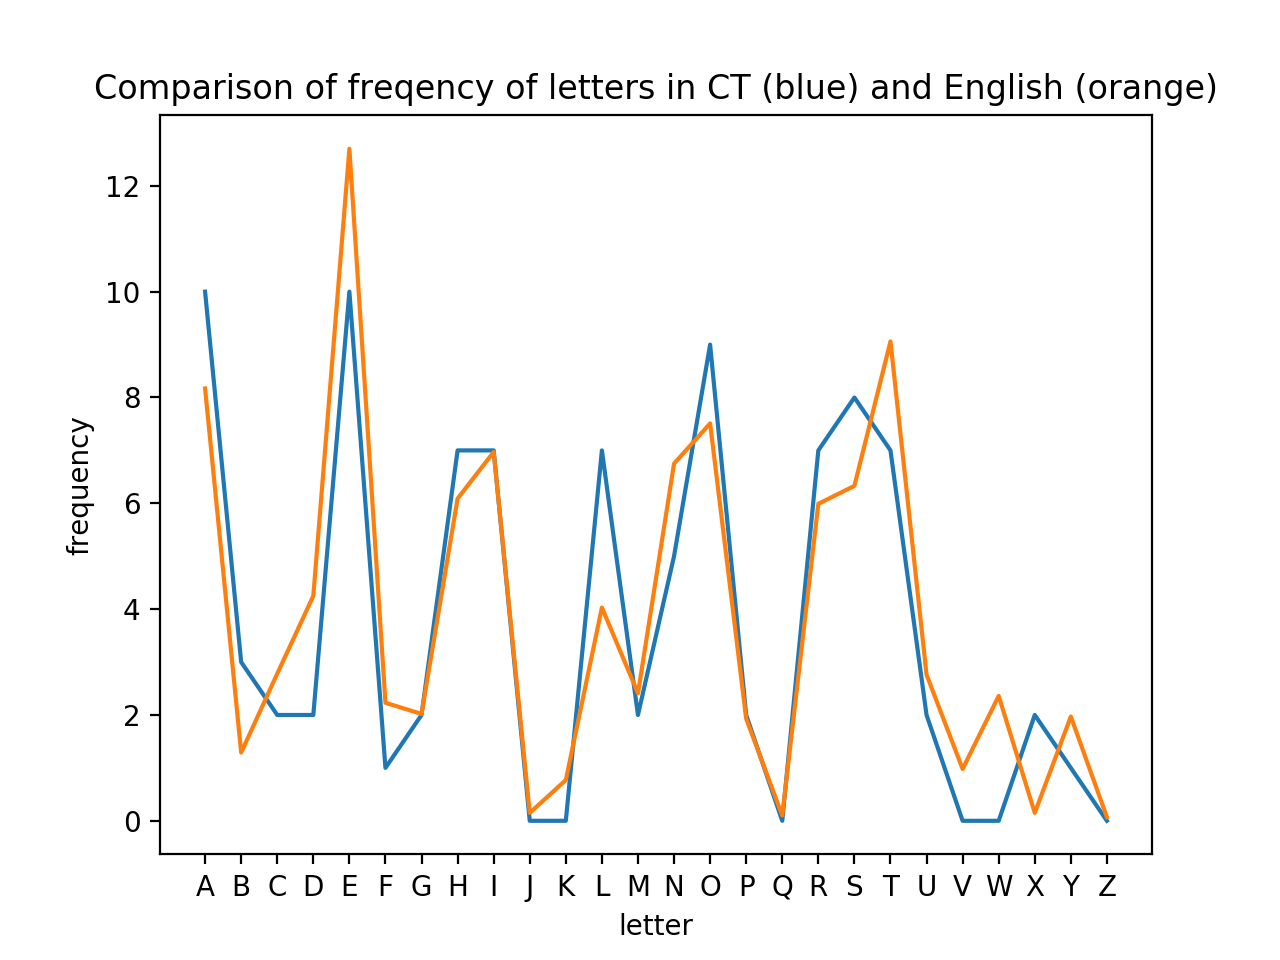
\includegraphics[width = 12cm]{img/q3freq}
			\captionsetup{width = 13cm}
			\caption{Frequency Analysis of the Ciphertext (CT) in comparison to text in the English language. The two graphs are very similar in shape and therefore the cipher method using is likely to be a transpositional cipher.}
			\label{q3freq}
		\end{figure}

	Two main methods exist for transposition ciphers; the simplest being the Rail Fence Cipher, and the other being the Columnar Transposition Cipher. The method of approach used here began by exploring the Rail Fence Cipher method. A script, \url{railTest.py} was developed to show that the implementation would allow messages to be both encrypted and decrypted using the Rail Fence Cipher. The decryption methods from this script were then used in another script, \url{rail.py} to Brute Force all possible combinations of the plaintext for the given ciphertext.
	
	The ciphertext has a length of 96 characters and therefore there could be up to 95 rails used in this cipher mode. The \url{rail.py} script produced all the possible plaintexts when using any number of rails between 2 and 95. The result of this showed that the ciphertext had not used the Rail Fence Cipher as the decrypted messages held no useful information. Therefore the Columnar Transposition Cipher was then attempted as a method to decrypt the plaintext.
	
	A python script was developed to once again Brute Force all possible combinations of the ciphertext to generate the potential plaintexts (\url{q3.py}). For this method a table is generated containing the ciphertext with a number of columns matching the length of the key being used. These columns are re-arranged using the alphabetical order of the word being used as the key. The Brute Force method employed therefore had to generate the possible tables for keys of various lengths and then try every possible combination when re-ordering the columns as to produce all possible plaintexts.
	
	The length of the message was 96 characters long and therefore potential key lengths (excluding those with length less than 3) were \url{3,4,6,8,12,16,24,32,48,96}. The developed script used two language recognition libraries to examine the plaintexts produced using the re-arrangement method of the columns. A set of rules were introduced using these libraries so that the number of plaintexts output was limited. This was required due to the increasing number of potential plaintexts for increasing key number as shown in Table \ref{q3brute} for key lengths of up to 8.
			
		\begin{table}[h]
			\centering
			\scriptsize
			\begin{tabular}{|| c | c | c ||}
			\hline
			Key Length & Calculation of Number of Plaintexts & Number of Plaintexts \\
			\hline \hline
			3 & $3! = 3\times2\times1$ & 6 \\
			\hline
			4 & $4! = 4\times3\times2\times1$ & 24 \\
			\hline
			6 & $6! = 6\times5\times4\times3\times2\times1$ & 720 \\
			\hline
			8 & $8! = 8\times7\times6\times5\times4\times3\times2\times1$ & 40320 \\
			\hline
			\end{tabular}
			\captionsetup{width = 12cm}
			\caption{Increasing number of plaintexts produced by the Brute Force method of decrypting the Columnar Transposition Cipher. The total number of columns in the transposition table is given by the length of the key and each column can then be re-arranged to generate a large number of permutations all providing unique potential plaintexts.}
			\label{q3brute}
		\end{table}

	Two language libraries were used as each provided different analysis methods, neither of which was perfect, but together they provided a fairly successful method for detecting english words in the deciphered plaintexts. A filtering process implemented using language detection meant that only 48 potential plaintexts were output having run the \url{q3.py} script. These were then examined and the plaintext was found in amongst this list. The decrypted plaintext is found in Section \ref{Solution for Cipher 3} and the scripts used in this section in Appendix \ref{Code for solving Cipher 3}.
	
% Appendices
\pagebreak
\pagenumbering{roman}
\begin{appendices}

	\section{Code for solving Cipher 1} \label{Code for solving Cipher 1}
		{\bfseries{indexOfCoincidence.py}}
		\lstinputlisting{code/q1/indexOfCoincidence.py}
		\newpage
		
		{\bfseries{caesar.py}}
		\lstinputlisting{code/q1/caesar.py}
		\newpage
		
		{\bfseries{q1.py}}
		\lstinputlisting{code/q1/q1.py}
		\newpage
		
		{\bfseries{q1.py Command Line Output}}
		\lstinputlisting{code/q1/vigenere.txt}

	\newpage	
	\section{Code for solving Cipher 2} \label{Code for solving Cipher 2}
		{\bfseries{q2.py}}
		\lstinputlisting{code/q2/q2.py}
		\newpage

		{\bfseries{q2.py Command Line Output}}
		\begin{figure*}[h]
			\centering
			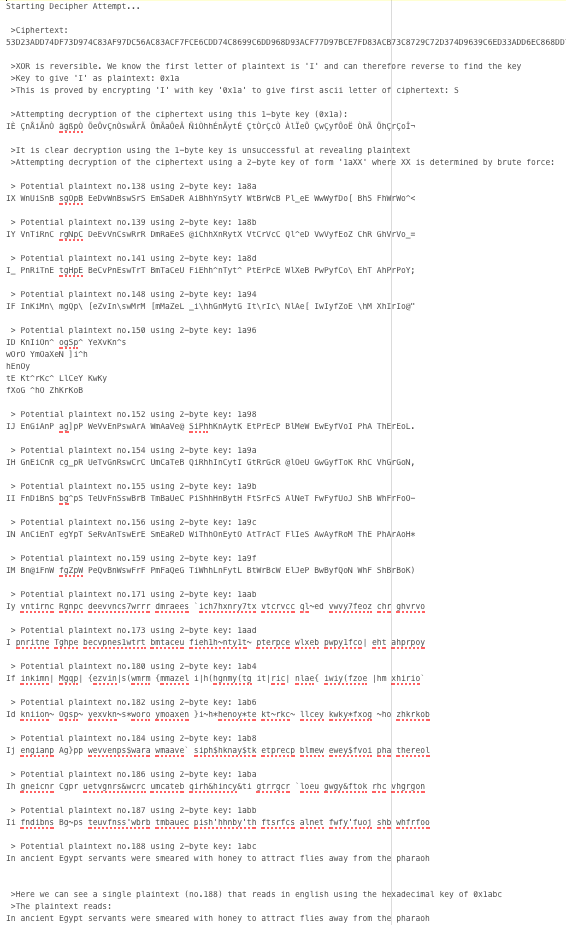
\includegraphics[width = 12cm]{img/xorLog}
		\end{figure*}

	\newpage
	\section{Code for solving Cipher 3} \label{Code for solving Cipher 3}		
		{\bfseries{railTest.py}}
		\lstinputlisting{code/q3/railTest.py}
		\newpage
		
		{\bfseries{rail.py}}
		\lstinputlisting{code/q3/rail.py}
		\newpage

		{\bfseries{q3.py}}
		\lstinputlisting{code/q3/q3.py}
		\newpage
		
		{\bfseries{q3.py Command Line Output}}
		\lstinputlisting{code/q3/columnar.txt}
	
	\newpage
	\section{Word Count} \label{Word Count}
		The total word count for each section was found using Texcount and the output is below showing that no individual section of the report is longer than the 500 word limit.
		
		\begin{lstlisting}
File: Crypto.tex
Encoding: ascii
Words in text: 1667
Words in headers: 39
Words outside text (captions, etc.): 207
Number of headers: 11
Number of floats/tables/figures: 7
Number of math inlines: 2
Number of math displayed: 1
Subcounts:
  text+headers+captions (#headers/#floats/#inlines/#displayed)
  88+1+0 (1/0/0/0) Section: Outline} \label{Outline
  66+4+0 (1/0/0/0) Section: Solution for Cipher 1} \label{Solution for Cipher 1
  500+3+85 (1/2/0/1) Section: Cipher 1 Cryptanalysis} \label{Cipher 1 Cryptanalysis
  19+4+0 (1/0/0/0) Section: Solution for Cipher 2} \label{Solution for Cipher 2
  423+3+35 (1/2/2/0) Section: Cipher 2 Cryptanalysis} \label{Cipher 2 Cryptanalysis
  24+4+0 (1/0/0/0) Section: Solution for Cipher 3} \label{Solution for Cipher 3
  497+3+87 (1/2/0/0) Section: Cipher 3 Cryptanalysis} \label{Cipher 3 Cryptanalysis
  7+5+0 (1/0/0/0) Section: Code for solving Cipher 1} \label{Code for solving Cipher 1
  5+5+0 (1/1/0/0) Section: Code for solving Cipher 2} \label{Code for solving Cipher 2
  7+5+0 (1/0/0/0) Section: Code for solving Cipher 3} \label{Code for solving Cipher 3
  31+2+0 (1/0/0/0) Section: Word Count} \label{Word Count
		\end{lstlisting}
	
\end{appendices}

\end{document}